\chapter{Monte Carlo event generation}
\label{ch:mc}

% need simulation to compare experimental measurements, i.e. event counts, to predictions
% probabilistic - many parts untractable (hadronization, detector response, etc), huge phase space
% MC simulation: always good-ish convergence even with large phase space
% can be computationally expensive
% chain of simulation tools: ME - parton shower - hadronization & decay, MPI - pileup - detector & trigger simulation

In order to test the Standard Model or extract any of its parameters at the LHC, one requires a prediction of proton-proton scattering which can be directly compared to the experimental data recorded by the detectors in the form of collision events. This is, in general, a very complex task consisting of many different subprocesses and physical scales, which are illustrated in \cref{fig:mc:sketch}. The generation starts with the hard parton scattering, then continues with the emission of additional gluon and quark radiation, effects of interactions of other partons in the colliding protons, the creation of color-neutral hadrons from gluons and quarks, interactions between other protons in the same bunch, and ends with the simulation of the different subdetectors and triggers. Many of these processes are not only probabilistic, but intractable through direct analytical or numeric integration due to the large phase space and the complexity of the problems involved. To compare to recorded events, one further requires a prediction that is fully differential in all variables explicitly and implicitly considered in an experimental analysis.

\begin{figure}[!t]
    \centering
    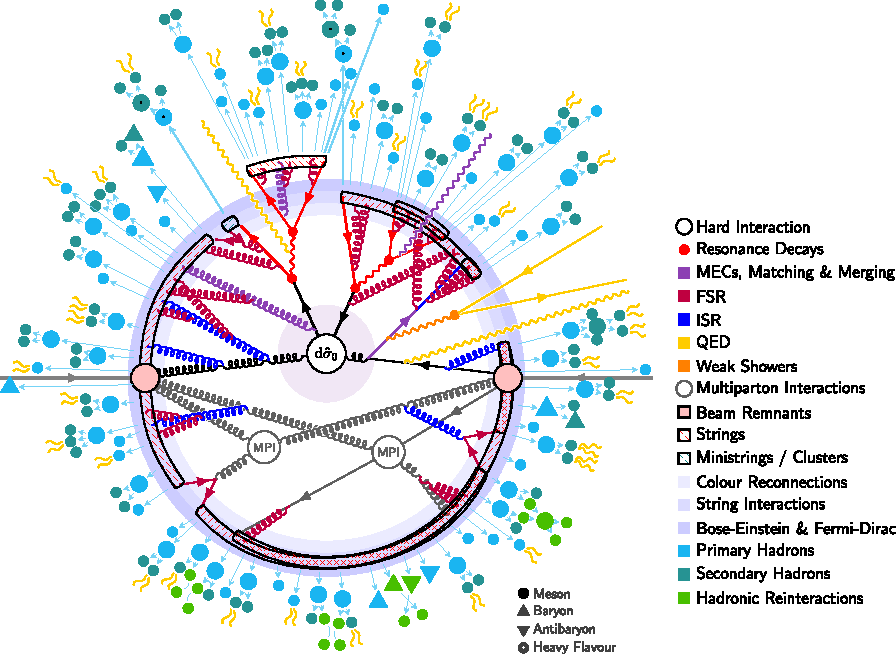
\includegraphics[width=\textwidth]{figures/mc_sketch.pdf}
    \caption{\textbf{Illustration of MC generation}. An illustration of the different subprocesses and scales involved in MC generation, starting from the hard scattering in the center (white circle) and ending with physical hadrons at the outside, for the example of a \pptt event with fully hadronic decays as simulated in \pythia. \textit{Figure taken from \citere{Pythia:2022}}.}
    \label{fig:mc:sketch}
\end{figure}

For this purpose, the Monte Carlo (MC) method is used. Here, it amounts to randomly sampling an event from the phase space of the starting distribution - in this case, the hard scattering - and then passing it through a chain of simulation tools for the remaining steps until one arrives at an event that is directly comparable to events recorded experimentally. %Events are discarded if, based on the simulation, they are expected to not be detectable experimentally, e.g. because they fail the trigger requirements.
This method is advantageous in that the numerical error in an arbitrary region of phase space always scales with $1/\sqrt{N}$, where $N$ is the total number of events produced, independently of the dimensionality of the problem. Thus, getting a numerically accurate prediction is mostly a matter of producing a sufficient number of MC events.

In this chapter, the different tools used in the CMS simulation chain are discussed. A focus is laid on the hard scattering or matrix element generators (\cref{sec:mc:me}) as well as the parton showering (\cref{sec:mc:showering}) since these are the focus of the studies presented in \cref{ch:bb4l}, while interactions with other partons in the colliding protons (``multi-parton interactions'', \cref{sec:mc:mpi}), hadronization (\cref{sec:mc:hadronization}), interactions between other protons in the same bunch (``pileup'', \cref{sec:mc:pileup}), as well as the detector and trigger simulation (\cref{sec:mc:detector}) are only briefly touched upon. 

\section{Matrix Element generators}
\label{sec:mc:me}

% generate hard scattering
% ME element, phase space factors
% convolution with PDF, factorization theorem of QCD
% higher orders in QCD: real + virtual corrections
% renormalization & factorization scales: chosen heuristically, represent missing knowledge (of non-pert. / higher orders respectively)

At the LHC, protons are collided with large center-of-mass energies of multiple TeV. Because protons are not fundamental particles, but bound states of QCD consisting of quarks and gluons (partons) which cannot be perturbatively described from first principles (cf. \cref{sec:theory:qcd}), providing accurate predictions for proton-proton collisions is generally a very challenging task. For the specific case of hard scattering processes, i.e. processes in which the particles in the final state $X$ have large transverse momenta, one can employ the factorization theorem of QCD~\cite{Peskin:1995ev}:

\begin{equation}
\label{eq:mc:sigmahad}
    \sigma (\mathrm{pp} \rightarrow X) = \int_{0}^{1} dx_1 \int_{0}^{1} dx_2 \sum_ {a,b} f_a (x_1, \mu_F) f_b (x_2, \mu_F) \, \hat{\sigma} (a (x_1 P) + b (x_2 P) \rightarrow X)
\end{equation}

\noindent where $P$ is the incoming momentum of the protons, assumed to be purely longitudinal and thus $P = \sqrt{s}/2$, and the sum runs over all possible combinations $a,b$ of initial state partons. This formula factorizes the total hadronic cross section into two parts: The partonic cross section $\hat{\sigma} (a + b \rightarrow X)$ describes the scattering of two partons at high energies, and can be computed perturbatively in \alphas due to asymptotic freedom of QCD. The functions $f_a(x, \mu_F)$  on the other hand are the parton distribution functions (PDFs) and describe the probability of finding a parton of type $a$ with momentum fraction $p_a / P = x$ in the proton structure~\cite{Peskin:1995ev}. Since they probe low momentum scales where \alphas is large, they cannot be computed perturbatively and instead need to be measured experimentally. In addition to $x$, they also depend on the factorization scale $\mu_F$, which is the energy scale defining the separation between hard (perturbative) and soft (non-perturbative) QCD. It is typically set to be equal to the characteristic energy of the incoming partons, e.g. half the partonic invariant mass. In contrast to the dependence on $x$, the dependence on $\mu_F$ is a prediction of QCD and follows from the DGLAP equations~\cite{Altarelli:1977zs,Skands:2012ts}.

%At the LHC, where ultra-relativistic particles with the same mass are collided, the differential hard scattering cross section in the hadronic center-of-mass frame for a given set of final state particles $f$ with momenta $p_f$ can in general be written as~\cite{Peskin:1995ev}

The partonic cross section can further be written differentially as~\cite{Peskin:1995ev}

\begin{equation}
    d \hat{\sigma} (a b \rightarrow X) = \frac{1}{2 \hat{s}} \left( \prod_f \frac{d^3 p_f}{(2\pi)^3} \frac{1}{2 E_f} \right) \, \left| \mathcal{M} (a b \rightarrow 
    X ) \right|^2 \, (2\pi)^4 \delta^{(4)} \left( \sum_f p_f \right)
\end{equation}

\noindent where $\hat{s} = x_1 x_2 s$ is the partonic center-of-mass energy squared, the term in the brackets refers to the integral over the final state phase space and depends only on the properties of the final state particles $f$, the $\delta$ function encodes energy and momentum conservation, and only the scattering matrix element $\mathcal{M}$ depends on the details of the interaction mediating the considered process.

Events are now generated by drawing randomly from the full kinematically allowed final state phase space, as well as from the PDFs characterizing the initial state, and keeping them with a probability proportional to the corresponding hadronic cross section according to \cref{eq:mc:sigmahad}. The partonic cross section here is usually known analytically, though for complex processes (especially at NLO or higher) it usually leads to complicated expressions requiring the use of computer algebra. The PDFs, based on fits to experimental data, are usually tabulated and interpolated; in this work, the NNPDF~3.1 PDF set is most commonly used for this purpose~\cite{NNPDF:2017mvq}. In practice, codes usually employ an adaptive sampling algorithm to enhance the fraction of events that pass and thus speed up the calculation, see e.g. \citere{Maltoni:2002qb}.

\subsection{Higher orders in QCD}

ME generators exist at LO, NLO, and (approximate) NNLO in QCD, all of which are used at different points in this work. For NLO and NNLO processes, care must be taken to cancel ultraviolet (UV) as well as infrared (IR) divergences that appear in the integration of the matrix element. The former is done in the framework of renormalization, which usually introduces a dependence on an additional scale, the renormalization scale $\mu_R$. Similar to $\mu_F$, it is typically set to the energy scale of the process, and, since the dependence is expected to vanish at infinite order in QCD, variations of $\mu_R$ and $\mu_F$ are often used to asses the size of uncertainties due to missing higher orders~\cite{Schwartz:2014sze}\footnote{Using $\mu_R$ and $\mu_F$ variations as estimates of missing higher order uncertainties, while common, can only give a rough estimate of the magnitude of missing higher order contributions and does not truly give information about shape deficiencies in differential distributions. A recent, more thorough approach are \textit{theory nuisance parameters} quantifying the uncertainty in specific parts of the theory calculation~\cite{Tackmann:2024kci}. This method has however not yet been extended to \ttbar production and is thus not considered here.}.

IR divergences, on the other hand, arise in two circumstances: first, when the momenta of massless particles in loop diagrams, such as gluons or light quarks, approach zero; and second, when a real massless particle is emitted such that it is soft or collinear with respect to the emitter. These two contributions from real and virtual IR divergences need to be canceled with each other to obtain a finite result. As a result, NLO calculations for the final state $X$ will always need to also take into account the final state $X+j$, where $j$ can be a gluon or light quark~\cite{Nason:2012pr}. 

In an analytical (i.e. non-MC) fixed-order calculation, this cancellation can in principle be performed directly by summing the real and virtual contributions to an observable of interest before the numerical evaluation\footnote{In practice, subtraction methods are still commonly used for fixed-order calculations for numerical reasons, especially when the computation is automated for arbitrary processes~\cite{Skands:2012ts}.}. This is not possible in MC simulations, since the real and virtual contributions, which correspond to different final states, need to be kept as separate events. Instead, subtraction methods are commonly used, where counterterms canceling the divergences are respectively added to and subtracted from the real and virtual contributions. When considering both real and virtual events in an analysis, the counterterms cancel with each other and the full amplitude is recovered~\cite{Skands:2012ts}. A disadvantage of this method is that it can lead to negative weights for the events, since only the full amplitude, but not the real and virtual contributions on their own, are guaranteed to be positive definite. How significant this problem is in practice strongly depends on the method used and the process in question.

In this work, two different ME generators are used. The first is \amcatnlo, a general-purpose ME generator that can work both at LO and NLO~\cite{MG5aMCatNLO:2014}. It features fully automated computation of arbitrary processes in the SM or BSM, where the model is specified in the Universal FeynRules Output (UFO) format~\cite{Degrande:2011ua}. It is used in this work for both SM and BSM processes. 

The second ME generator used is \powheg Box (short for Positive Weighted Hardest Emission Generator), which is a generic framework for NLO and approximate NNLO generators~\cite{Powheg:2004,Powheg:2007,Powheg:2010}. In contrast to \amcatnlo, it is not automated, and requires the manual implementation of each process. Many processes are publicly available as part of the \powheg Box collection, and several are used in this work. Importantly, \pptt is generated at NLO with the \powheg Box process \hvq~\cite{Frixione:2007nw} in \cref{ch:ttxs,ch:ah,ch:alps}. %\powheg has the advantage that it generates (almost) only events with positive weights, while the subtraction procedure in \amcatnlo leads to a significant fraction of negative weights at NLO~\cite{Frixione:2002ik}, possibly leading to numerical instability in certain regions of phase space.
The two generators also differ in the scheme used to match to the parton shower, which is explained in the next section.

\subsection{ME generators for \ttbartitle}
\label{sec:mc:ttbar}

Throughout this work (\cref{ch:ttxs,ch:bb4l,ch:ah,ch:alps}), the \pptt process is mostly generated using the \powheg Box subprocess \hvq~\cite{Frixione:2007nw}. This generator employs the narrow-width approximation (NWA), which means that it treats the top quark as a stable particle with a fixed mass and zero width. It thus generates \pptt as a $2 \rightarrow 2$ process, with the top quarks in the final state, at NLO in QCD. As with all \powheg Box processes, it is intended to be matched to a parton shower (cf. next section). 

However, in practice the top quark is unstable, i.e. it has a finite width, and decays immediately to a W boson and a b quark (cf. \cref{sec:theory:ttbar}). In \hvq, the modeling of the decay is done approximately in a second step after the production of \ttbar. This proceeds as follows~\cite{Frixione:2007zp,Artoisenet:2012st}: 
for each event, generated at the level of stable \ttbar, the allowed decay phase space of both top quarks is randomly and uniformly sampled, i.e. random three-momenta are drawn in the top or antitop rest frame for the possible decay products ($b \ell \nu$ or $b q \bar{q}$). The full matrix elements for the $2 \rightarrow 6$ process including decays, e.g. $\mathrm{pp} \rightarrow \bbllnunu$ for a dilepton decay, are now evaluated at LO in QCD for the randomly drawn three-momenta of the decay products. The three-momenta are now kept with a probability proportional to the matrix element; otherwise, they are thrown away and the decay procedure is repeated.\footnote{A very similar algorithm is implemented in the code \textsc{MadSpin}~\cite{Artoisenet:2012st}, and the algorithm is sometimes known as the MadSpin algorithm.}

This algorithm is computationally efficient, since only the $2 \rightarrow 2$ production matrix element needs to be computed (i) at NLO and (ii) during the event generation process. It furthermore has the advantage that it includes \ttbar spin correlations (cf. \cref{sec:theory:ttbarspin}), at least at LO, since the decay of t and \tbar are treated at the same time (as opposed to decaying t and \tbar independently). 

However, it does not capture finite width effects since the top quarks are considered stable during event generation. In \hvq, it is possible to alleviate this somewhat by reshuffling the momenta of the decayed \ttbar events such that the invariant mass of the t and \tbar decay products follows a simple Breit-Wigner distribution~\cite{Artoisenet:2012st}. This option is used in this work everywhere \hvq is considered. It still represents an ad-hoc procedure with no guarantee to reproduce the true top quark line shape at any order in QCD. 

To improve on this, one needs to consider the full $2 \rightarrow 6$ process without explicitly splitting into production and decay. Among others, this is done at NLO in QCD for the dilepton final state by a different \powheg Box subprocess called \bbfourl ~\cite{Jezo:2016ujg}. In \cref{ch:bb4l}, \bbfourl is discussed in detail and validated in the context of CMS simulation, and it is applied to the modeling of the \ttbar production threshold in \cref{sec:ah:gennps}.

\section{Parton showers and matching}
\label{sec:mc:showering}

% problem: radiation of gluons in QCD
% coupling constant is large - happens often
% confinement - free gluons and quarks are not physical, need to hadronize
% but hadronization happens at low scales: Lambda_QCD
% idea: start with hard scattering, evolve down to hadronization scale by radiating gluons off quarks & splitting gluons into gg or qq 
% probability of splitting at a certain scale given by matrix elements - perturbative in principle!
% but: collinear & infrared singularities

The output of ME generators are events whose final states typically involve quarks and gluons with high momenta. Formally, such computations are accurate to some fixed order in \alphas at which the calculation was performed, and all further emissions of gluons, as well as splittings of gluons into quark-antiquark-pairs, is suppressed by additional powers of \alphas. 
However, the matrix elements for such splittings become singular in the limit that the emitted partons are \textit{soft} and/or \textit{collinear} to the emitting particle, leading to IR divergences. For initial state radiation, the divergences can be regulated by absorbing them in renormalized PDFs, from which the DGLAP equations can be derived~\cite{Skands:2012ts,Schwartz:2014sze}. They still lead to large corrections for each additional soft or collinear splitting considered, 
proportional to $\alphas \log( \hat{s} / \Lambda_{\mathrm{QCD}}^2)$, where $\Lambda_{\mathrm{QCD}} \approx \SI{250}{\MeV}$ is the scale at which QCD becomes nonperturbative. This term is of order 1 and thus spoils the convergence of the perturbative series if it is cut off at a fixed order in \alphas~\cite{Peskin:1995ev,Skands:2012ts}.
Physically, this corresponds to the emission of many further partons besides the one or two considered at NLO or NNLO, which are not captured by the matrix element at a fixed order in QCD.

A way to approximately incorporate these emissions is by using parton showers. %The idea of a parton shower is to successively generate all real emissions and splittings down to the scale of $\Lambda_{\mathrm{QCD}}$.
For a parton associated with some scale $Q_0$, the probability for no splitting to occur above some scale $Q$ (with $Q < Q_0$) is called the \textit{Sudakov factor} $\Delta(Q_0,Q)$. Because the structure of the IR singularities in QCD is universal, i.e. depending only on the types of particles in the splitting but not the rest of the process, its leading-logarithmic behavior can be computed from the matrix elements of $\mathrm{q \rightarrow qg}$ and $\mathrm{g \rightarrow \qqbar}$ splittings (the \textit{splitting kernels}).
The parton shower algorithm now iteratively draws random numbers from this distribution, thus generating real emissions and splittings with successively lower scales $Q$ down to $\Lambda_{\mathrm{QCD}}$. In practice, the Sudakov factor usually contains additional terms beyond the leading-logarithmic behavior depending on the details of the algorithm~\cite{Skands:2012ts}.

%where every splitting happens with a probability proportional to \alphas and the corresponding logarithm. 
The scale $Q$ which determines in which order the splittings are performed is also called the \textit{ordering variable}, and its form can be freely chosen as long as it correctly captures the soft and collinear singularities. Two common choices are the transverse momentum of the emission (\pt-ordered shower) or the emission angle respective to the emitting particle (angular-ordered shower). The result of either choice is an effective resummation of the logarithms associated to each emission, which is why parton showers are said to be leading-log (LL) accurate for certain observables.

The main parton shower used in this work is a \pt-ordered dipole shower, included as part of the \pythia multi-purpose event generator~\cite{Pythia:2015,Pythia:2022}. It works by collecting quark-antiquark pairs into color dipoles, which radiate gluons together so that the recoil is distributed between the quarks. Here, it is mostly used by matching it to the ME generators described in \cref{sec:mc:me}. This is usually trivial at LO: the parton shower simply starts from the final state as given by the ME generator.

At NLO or higher, however, care must be taken that there is no double-counting between the additional real emissions in the final state of the ME generator (e.g. \amcatnlo or \powheg Box) and the emissions of the shower (e.g. \pythia), as well as between the virtual corrections that are exact in the ME generator and approximated in the shower~\cite{Skands:2012ts}. Several matching schemes exist to solve this issue. In this work, the MC@NLO and POWHEG schemes are used and briefly explained in the following.

In the MC@NLO scheme~\cite{Frixione:2002ik}, as implemented in \amcatnlo, the double-counting is corrected for using another subtraction scheme: During the generation of the real and virtual correction terms in the matrix elements, the approximate corrections that would be used in the parton shower are subtracted from the squared amplitude. When the events generated in this way are then showered, the approximate correction terms are effectively added back, so that formally the exact result is recovered at NLO accuracy. This strategy is conceptually simple and easy to generalize (and thus automatize, as done in \amcatnlo). However, at phase-space points where the approximate terms are larger than the exact ones, it inherently results in events with negative weights, which can greatly increase the MC statistics required.

In the POWHEG scheme~\cite{Powheg:2004,Powheg:2007}, as used in the \powheg Box, the fraction of negative weights is greatly reduced by always generating the first real emission in the ME generator, so that the real emission term is already exact, and then only subtracting the approximate virtual correction term. The parton shower then needs to only generate the second-hardest and higher emissions, which is typically achieved by starting the shower evolution at the scale of the first, ME-level emission (sometimes called ``wimpy shower'').

%At NLO or higher, however, the additional emissions in the final state of the ME generator that need to be inherently included to regularize IR singularities would lead to double-counting if the parton shower is run in a naive way. 
%To prevent this, the most common strategy in \pythia is to start both initial state and final state parton showers at the scale of the ME-level emission (sometimes called ``wimpy shower'').

This approach assumes that the scale definitions in the ME generator and the parton shower are identical, which in general will not always be the case. In particular, for the important case of \powheg matched to \pythia, used in this work for the simulation of \pptt, there is a mismatch in the scales which might lead to double-counting. A more refined approach here is to use a vetoed shower: the shower evolution is started at the kinematically allowed limits and evolves downwards as usual, ordered by the scale as defined by \pythia. For the first emission the scale is then recomputed according to the \powheg definition, and it is vetoed and re-showered if this scale is higher than the one in the ME.

A further improvement in the accuracy of the MC prediction can be achieved by generating any number of additional jets in the matrix element at either LO or NLO, so that these jets are described exactly by the ME generator instead of approximately by the shower. This, however, requires complex matching procedures, such as MLM matching~\cite{Mangano:2006rw} for LO and FxFx matching~\cite{Frederix:2012ps} for NLO matrix elements. In this work, both schemes are only used tangentially for either background processes in \cref{ch:ttxs} or an alternative \ttbar prediction in \cref{ch:ah}.

More complicated procedures have to be invoked in the case that the ME contains more than one real emission. This case is studied in detail for the ME generator \bbfourl in \cref{ch:bb4l}. Furthermore, besides \pythia, the multi-purpose generator \herwig~\cite{Bellm:2015jjp,Bahr:2008pv} is considered in parts of \cref{ch:ah}, and briefly described there.

%In addition to \pythia, the alternative multi-purpose generator \herwig~\cite{Bellm:2015jjp,Bahr:2008pv} is considered in parts of \cref{ch:ah}. The default shower model in \herwig is angular-ordered, in contrast to the \pt-ordered dipole shower of \pythia. Furthermore, \herwig employs a cluster hadronization model~\cite{Webber:1983if} instead of string hadronization. In \cref{sec:ah:gennps}, a brief comparison of \ttbar production matched to \pythia or \herwig is performed in the context of the search for \ttbar bound states.

%\todo{remove redundant info from bb4l part}

% for NLO ME: already emission in ME
% needs to be matched to shower to not double count
% details depend on the exact algorithms of ME generator and shower

\section{Multi-parton interactions}
\label{sec:mc:mpi}

In addition to the hard scattering, additional soft QCD interactions might occur between the other partons in the two colliding protons. This is referred to as multi-parton interactions (MPI) or underlying event (UE). It is handled by \pythia based on heuristic models, interleaved with the parton shower. In general, MPI parameters need to be tuned to experimental data. This was done by the \pythia authors, such as the different versions of the Monash tune~\cite{Skands:2014pea}, and building on top of this by the CMS collaboration in the form of the CP tune family, most recently the CP5 tune~\cite{CMS:GEN-17-001}. Both tunes are based on a large data set of $e^+e^-$, $ep$, $p\bar{p}$, and $pp$ collision data from many different experiments. The CP5 tune will be used in all parts of this work.

\section{Hadronization}
\label{sec:mc:hadronization}

In the course of the MPI-interleaved parton shower, the gluons and quarks gradually become softer until the parton shower is stopped at an arbitrary cutoff scale, which should lie slightly above the energy scale $\mathcal{O}(\Lambda_{\mathrm{QCD}})$ at which QCD becomes non-perturbative.
The physics below this scale, namely 
%The result of the MPI-interleaved parton shower consists of a collection of bare quarks and gluons at energies of $\mathcal{O}(\Lambda_{\mathrm{QCD}})$, at which QCD becomes non-perturbative. 
the hadronization of these quarks and gluons into hadrons as well as their subsequent decays, thus needs to be described heuristically.

For most of this work, this is done using the Lund string fragmentation model~\cite{Andersson:1983ia,Sjostrand:1984ic}, again implemented in \pythia. In this model, the strong force between a quark and an antiquark of opposite color is modeled as a string in space-time, standing in for a three-dimensional flux tube. The energy stored in the string is proportional to its length, consistent with the long-distance behavior of the QCD potential observed e.g. in lattice QCD. Hard gluons can be accommodated in this model as kinks in the string, i.e. for a $q\bar{q}g$ state, the $q$ and $\bar{q}$ are connected through the gluon instead of directly.

As the quarks move apart, the energy stored in the string increases, until it is large enough that the string fragments by creating an additional $q\bar{q}$ pair from the vacuum (cf. \cref{sec:theory:qcd}). This repeats if the energy in the resulting strings is still large enough. Otherwise, the low-mass $q\bar{q}$ pair is considered a meson, based on the flavors of its constituents. This way, only color-neutral particles are present after hadronization, as required by confinement (cf. \cref{sec:theory:qcd}). In its purest form, this model has only two free parameters which parameterize the distribution of the momentum fraction of the $q\bar{q}$ pair in each fragmentation. However, in order to correctly describe e.g. flavor composition and \pt spectra of jets, many more parameters are usually needed. For more details on string fragmentation in \pythia, see e.g. \citere{Pythia:2022}. Similar to MPI, hadronization parameters need to be tuned to data, and are also included in the Monash and CP5 tunes.

One shortcoming of the default MPI and hadronization models is that both work in the leading color (LC) approximation, i.e. in the limit of a large number of QCD colors ($N_c \rightarrow \infty$). This simplifies the models greatly because the chance of two unrelated color lines sharing the same color becomes infinitesimally small. Corrections to this approximation are typically of order $1/N_c^2 = 1/9$, and can be done via color reconnection (CR), for which different models exist, see e.g. \citeres{Argyropoulos:2014zoa,Christiansen:2015yqa}. The difference between different models is often considered a source of uncertainty in measurements, such as in \cref{sec:ttxs:systematics,sec:ah:systs}, and can be a limiting factor for some analyses (e.g. top quark mass measurements~\cite{CMS:TOP-20-008,ATLAS:2025bpp}).

Finally, decays of produced unstable hadrons, including possible decay chains, are also handled by \pythia. Branching ratios are taken from experimental measurements where available, and predicted from heuristic models where not, see e.g. \citere{Pythia:2022}.

\section{Pileup}
\label{sec:mc:pileup}

At the currently achieved instantaneous luminosities, the proton bunches colliding at the LHC contain more than $10^{11}$ protons on average (cf. \cref{sec:methods:lhc}). Because of this large number, it is expected that a single collision event contains interactions between more than one pair of protons from the two colliding bunches. This is known as pileup. It differs from MPI, in which the different interactions are between multiple partons in the same proton and are thus correlated from a QFT perspective, while different pileup interactions are in principle independent from each other. In Run~2, the average number of pileup interactions per bunch crossing ranged from 23-32 depending on the era of data taking~\cite{CMS:2020ebo}, while it is 40 or higher in Run~3.

In simulation, pileup interactions are considered by mixing the generated hard interaction process with a dedicated sample of purely soft-QCD interactions, also generated in \pythia. The probability distribution of the number of pileup interactions is an input to this procedure, and is typically corrected after the generation is finished by reweighting in a suitable variable. In \cref{sec:ttxs:scalefactors}, an experimental approach to this problem is taken by correcting experimentally accessible pileup-related parameters directly to data. In \cref{sec:ah:expcorrs}, on the other hand, the distribution of the true number of interactions is instead reweighted based on a theory prediction, using the measured total inelastic cross section and integrated luminosity as inputs~\cite{CMS:LUM-17-003}.

\section{Detector and trigger simulation}
\label{sec:mc:detector}

After the simulation of the interaction processes, the resulting collection of particles produced in an event is propagated to a full detector simulation using the program \textsc{Geant4}~\cite{GEANT4:2002}. 
%Based on the output of this simulation, the two tiers of trigger systems are similarly simulated using in-house tools. 
The result is a set of detector information from all subdetectors as well as the outputs of different triggers, similar to true experimental data, and so it can be passed to the different object reconstruction algorithms (cf. \cref{sec:methods:reco}) in the same way as the data. Events are then analyzed by comparing the reconstructed objects and quantities between data and simulation, ensuring a one-to-one comparison. Possible residual differences between data and simulation are often corrected for by applying calibration factors measured using well-known processes. The details of such calibrations will be explained in \cref{ch:ttxs,ch:ah} where relevant.